\documentclass[12pt, paper=a4]{article}
\usepackage[utf8]{inputenc}
\usepackage[german]{babel}
\usepackage{amsmath}
\usepackage{amssymb}
\usepackage{listings}
\usepackage{graphicx}
\usepackage{fancyhdr}

\author{Mareike Göttsch, 6695217, Gruppe 2\\Paul Hölzen, 6673477, Gruppe 1\\Sven Schmidt, 6217064, Gruppe 1}

\title{FGI 2 Hausaufgaben 3}

\rhead{M. Göttsch, G-2; P. Hölzen, G-1; S. Schmidt, G-1}
\pagestyle{fancy}
\begin{document}
\maketitle

\section*{Aufgabe 3.3}

\subsection*{1.}
Es sind \(L(A_1)=((a+c)b)^*\),\\ \(L(A_2)=((a+c)b^*(a+c)a^*b)^*((a+c)b^*(a+c)a^*)^+\),\\ 
	\(L^\omega(A_1)=((a+c)b)^\omega\) und \\
	\(L^\omega(A_2)=(((a+c)b^*(a+c))a^\omega+((a+c)b^*(a+c)a^*b)^\omega\)).\\
	
\subsection*{2.}	
	Per Konstruktion nach Satz 1.8 ergibt sich:\\
	\(Q=\{(q_0,z_0),(q_0,z_1),(q_0,z_2),(q_1,z_0),(q_1,z_1),(q_1,z_2)\}, Q^0=\{(q_0,z_0)\}, \\
	F=\{(q_0,z_2)\} \) und 
	\((q_0,z_0)\underrightarrow{a,c}(q_1,z_1), (q_0,z_1)\underrightarrow{a,c}(q_1,z_2), (q_0,z_2)\underrightarrow{a}(q_1,z_2),\\
	(q_1,z_1)\underrightarrow{b}(q_0,z_1), (q_1,z_2)\underrightarrow{b}(q_0,z_0)\) \\ 
	\\
	Daraus ergibt sich folgender Automat \(A_3\): \\
	\begin {figure}[h]
  		\centering 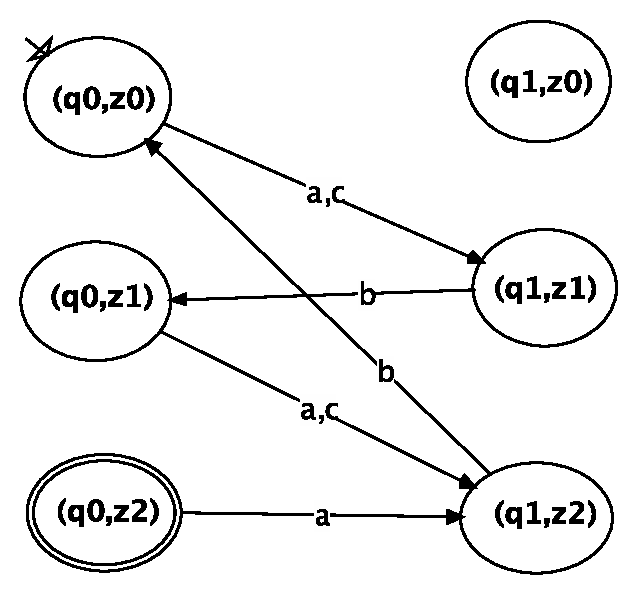
\includegraphics[width=0.5\textwidth]{A3}
	\end {figure}
	
\subsection*{3.}	
	Es sind \(L(A_3)=\emptyset\) und \(L^\omega(A_3)=\emptyset\),
	da der Endzustand \((q_0,z_2)\) nicht erreichbar ist.\\
	Es gilt \(L(A_3)=L(A_1)\cap L(A_2)\) und 
	\(L^\omega(A_3)\neq L^\omega(A_1)\cap L^\omega(A_2)=L^\omega(A_1)\).
	
\subsection*{4.}	
	Mit der Konstruktion nach Satz 1.21 ergibt sich:\\
	\(Q=\{(q_0,z_0,1),(q_0,z_0,2),(q_0,z_1,1),(q_0,z_1,2),(q_1,z_1,1),(q_1,z_1,2),(q_1,z_2,1),\\(q_1,z_2,2)\}\) 
	(es werden nur die initialen Zusammenhangskomponenten von \(A_3\) betrachtet),
	\(Q^0=\{(q_0,z_0,1)\}, F=\{(q_0,z_0,1),(q_0,z_1,1\} \) und \\
	\((q_0,z_0,1)\underrightarrow{a,c}(q_1,z_1,2),(q_0,z_0,2)\underrightarrow{a,c}(q_1,z_1,2),
	(q_0,z_1,1)\underrightarrow{a,c}(q_1,z_2,2),\\(q_0,z_1,2)\underrightarrow{a,c}(q_1,z_2,2),
	(q_1,z_1,1)\underrightarrow{b}(q_0,z_1,1), (q_1,z_1,2)\underrightarrow{b}(q_0,z_1,2),\\
	(q_1,z_2,1)\underrightarrow{b}(q_0,z_0,1),(q_1,z_2,2)\underrightarrow{b}(q_0,z_0,1)\).\\
	\\
	Daraus ergibt sich folgender Automat \(A_4\): \\
	\begin {figure}[h]
  		\centering 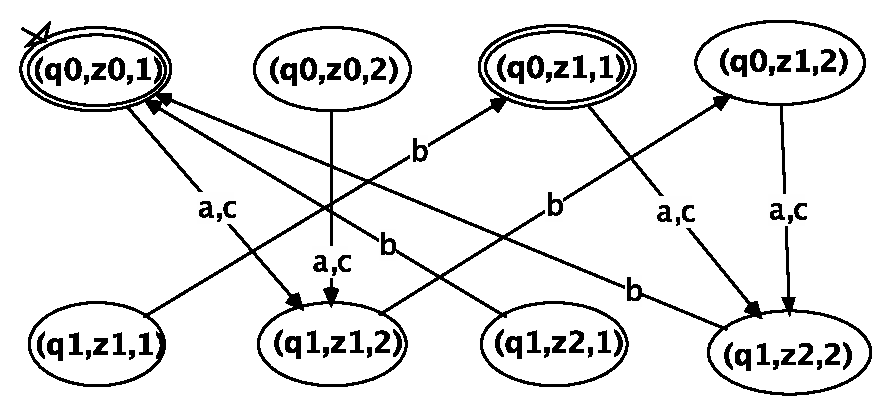
\includegraphics[width=0.6\textwidth]{A4}
	\end {figure}
	
\subsection*{5.}
	Es sind \(L(A_4)=((a+c)b(a+c)b)^*\) und \(L^\omega(A_4)=((a+c)b)^\omega\).
	Es ist \(L(A_1)\cap L(A_2)=\emptyset \neq L(A_4)\) und
	\(L^\omega(A_4) = L^\omega(A_1)\cap L^\omega(A_2)\).

\section*{Aufgabe 3.4}

\subsection*{1.}

	Die Transitionssysteme $TS_{1}$ und $TS_{2}$sind nicht bisimilar,
	da laut Definition das Element $\left(z_{2},p_{5}\right)$ in einer
	möglichen Bisimulationsrelation enthalten sein müsste. 

	Daraus folgt nach 
	\begin{gather*}
		p_{5}\stackrel{c}{\rightarrow}p_{6}\stackrel{b}{\rightarrow}p_{4}\stackrel{b}{\rightarrow}p_{5}\\
		\vdots\\
		z_{2}\stackrel{c}{\rightarrow}z_{0}\stackrel{b}{\rightarrow}z_{2}\stackrel{b}{\rightarrow}z!
	\end{gather*}


	dass das ebenfalls entahltene Element $\left(z_{2},p_{4}\right)$die
	Bedingung für eine Bisimulationsrelation nicht erfüllt.

	Die Transitionssysteme $TS_{1}$ und $TS_{3}$ sind bisimilar mit
	der folgenen Bisimulationsrelation 
	\[
		\text{\ensuremath{\mathscr{B}}}_{13}=\left\{ \left(z_{0},q_{0}\right),\left(z_{0},q_{4}\right),\left(z_{0},q_{8}		\right),...,\left(z_{1},q_{2}\right),\left(z_{1},q_{6}\right),...,\left(z_{2},q_{1}\right),\left(z_{2},q_{3}			\right),\left(z_{2},q_{5}\right),\left(z_{2},q_{7}\right),\left(z_{2},q_{9}\right),\right\} 
	\]


\end{document}
